%%
%% This is file `sample-lualatex.tex',
%% generated with the docstrip utility.
%%
%% The original source files were:
%%
%% samples.dtx  (with options: `sigconf')
%% 
%% IMPORTANT NOTICE:
%% 
%% For the copyright see the source file.
%% 
%% Any modified versions of this file must be renamed
%% with new filenames distinct from sample-lualatex.tex.
%% 
%% For distribution of the original source see the terms
%% for copying and modification in the file samples.dtx.
%% 
%% This generated file may be distributed as long as the
%% original source files, as listed above, are part of the
%% same distribution. (The sources need not necessarily be
%% in the same archive or directory.)
%%
%% Commands for TeXCount
%TC:macro \cite [option:text,text]
%TC:macro \citep [option:text,text]
%TC:macro \citet [option:text,text]
%TC:envir table 0 1
%TC:envir table* 0 1
%TC:envir tabular [ignore] word
%TC:envir displaymath 0 word
%TC:envir math 0 word
%TC:envir comment 0 0
%%
%%
%% The first command in your LaTeX source must be the \documentclass command.
\documentclass[sigconf]{acmart}
%% NOTE that a single column version is required for 
%% submission and peer review. This can be done by changing
%% the \doucmentclass[...]{acmart} in this template to 
%% \documentclass[manuscript,screen]{acmart}
%% 
%% To ensure 100% compatibility, please check the white list of
%% approved LaTeX packages to be used with the Master Article Template at
%% https://www.acm.org/publications/taps/whitelist-of-latex-packages 
%% before creating your document. The white list page provides 
%% information on how to submit additional LaTeX packages for 
%% review and adoption.
%% Fonts used in the template cannot be substituted; margin 
%% adjustments are not allowed.

%%
%% \BibTeX command to typeset BibTeX logo in the docs
\AtBeginDocument{%
  \providecommand\BibTeX{{%
    \normalfont B\kern-0.5em{\scshape i\kern-0.25em b}\kern-0.8em\TeX}}}

%% Rights management information.  This information is sent to you
%% when you complete the rights form.  These commands have SAMPLE
%% values in them; it is your responsibility as an author to replace
%% the commands and values with those provided to you when you
%% complete the rights form.

%% These commands are for a PROCEEDINGS abstract or paper.
%%\acmConference[Conference acronym 'XX]{Make sure to enter the correct
  %%conference title from your rights confirmation emai}{June 03--05,
  %%2018}{Woodstock, NY}
%
%  Uncomment \acmBooktitle if th title of the proceedings is different
%  from ``Proceedings of ...''!
%
%\acmBooktitle{Woodstock '18: ACM Symposium on Neural Gaze Detection,
%  June 03--05, 2018, Woodstock, NY} 


%%
%% Submission ID.
%% Use this when submitting an article to a sponsored event. You'll
%% receive a unique submission ID from the organizers
%% of the event, and this ID should be used as the parameter to this command.
%%\acmSubmissionID{123-A56-BU3}

%%
%% For managing citations, it is recommended to use bibliography
%% files in BibTeX format.
%%
%% You can then either use BibTeX with the ACM-Reference-Format style,
%% or BibLaTeX with the acmnumeric or acmauthoryear sytles, that include
%% support for advanced citation of software artefact from the
%% biblatex-software package, also separately available on CTAN.
%%
%% Look at the sample-*-biblatex.tex files for templates showcasing
%% the biblatex styles.
%%

%%
%% The majority of ACM publications use numbered citations and
%% references.  The command \citestyle{authoryear} switches to the
%% "author year" style.
%%
%% If you are preparing content for an event
%% sponsored by ACM SIGGRAPH, you must use the "author year" style of
%% citations and references.
%% Uncommenting
%% the next command will enable that style.
%%\citestyle{acmauthoryear}

%%
%% end of the preamble, start of the body of the document source.
\begin{document}

%%
%% The "title" command has an optional parameter,
%% allowing the author to define a "short title" to be used in page headers.
\title{Dead Code Elimination}

%%
%% The "author" command and its associated commands are used to define
%% the authors and their affiliations.
%% Of note is the shared affiliation of the first two authors, and the
%% "authornote" and "authornotemark" commands
%% used to denote shared contribution to the research.
\author{Robbie Hammond}
\affiliation{%
  \institution{Case Western Reserve Univerrsity, School of Engineering}
  \city{Cleveland}
  \state{Ohio}
  \country{USA}
  \postcode{44106}
}
\email{reh161@case.edu}

\author{Saketh Dendi}
\affiliation{%
  \institution{Case Western Reserve Univerrsity, School of Engineering}
  \city{Cleveland}
  \state{Ohio}
  \country{USA}
  \postcode{44106}
}
\email{ssd74@case.edu}

\author{Milo Cassarino}
\affiliation{%
  \institution{Case Western Reserve Univerrsity, School of Engineering}
  \city{Cleveland}
  \state{Ohio}
  \country{USA}
  \postcode{44106}
}
\email{mgc73@case.edu}
%%
%% By default, the full list of authors will be used in the page
%% headers. Often, this list is too long, and will overlap
%% other information printed in the page headers. This command allows
%% the author to define a more concise list
%% of authors' names for this purpose.
\renewcommand{\shortauthors}{Dendi, Hammond and Cassarino, et al.}

%%
%% The abstract is a short summary of the work to be presented in the
%% article.
\begin{abstract}
Dead code is a big contributor for arbitrarily large 
program sizes and slow speed, and our project attempts 
to create an optimization pass that is able to eliminate 
easy-to-find dead code. This paper outlines some of the 
high-level details of our implementation of the optimization pass. 
In addition, this paper outlines the results of the optimiztaion 
pass when ran on a number of simple test cases to demonstrate 
its effectiveness. 
\end{abstract}


%%
%% Keywords. The author(s) should pick words that accurately describe
%% the work being presented. Separate the keywords with commas.
\keywords{compiler optimization, dead code}

%% A "teaser" image appears between the author and affiliation
%% information and the body of the document, and typically spans the
%% page.
%%\begin{teaserfigure}
  %%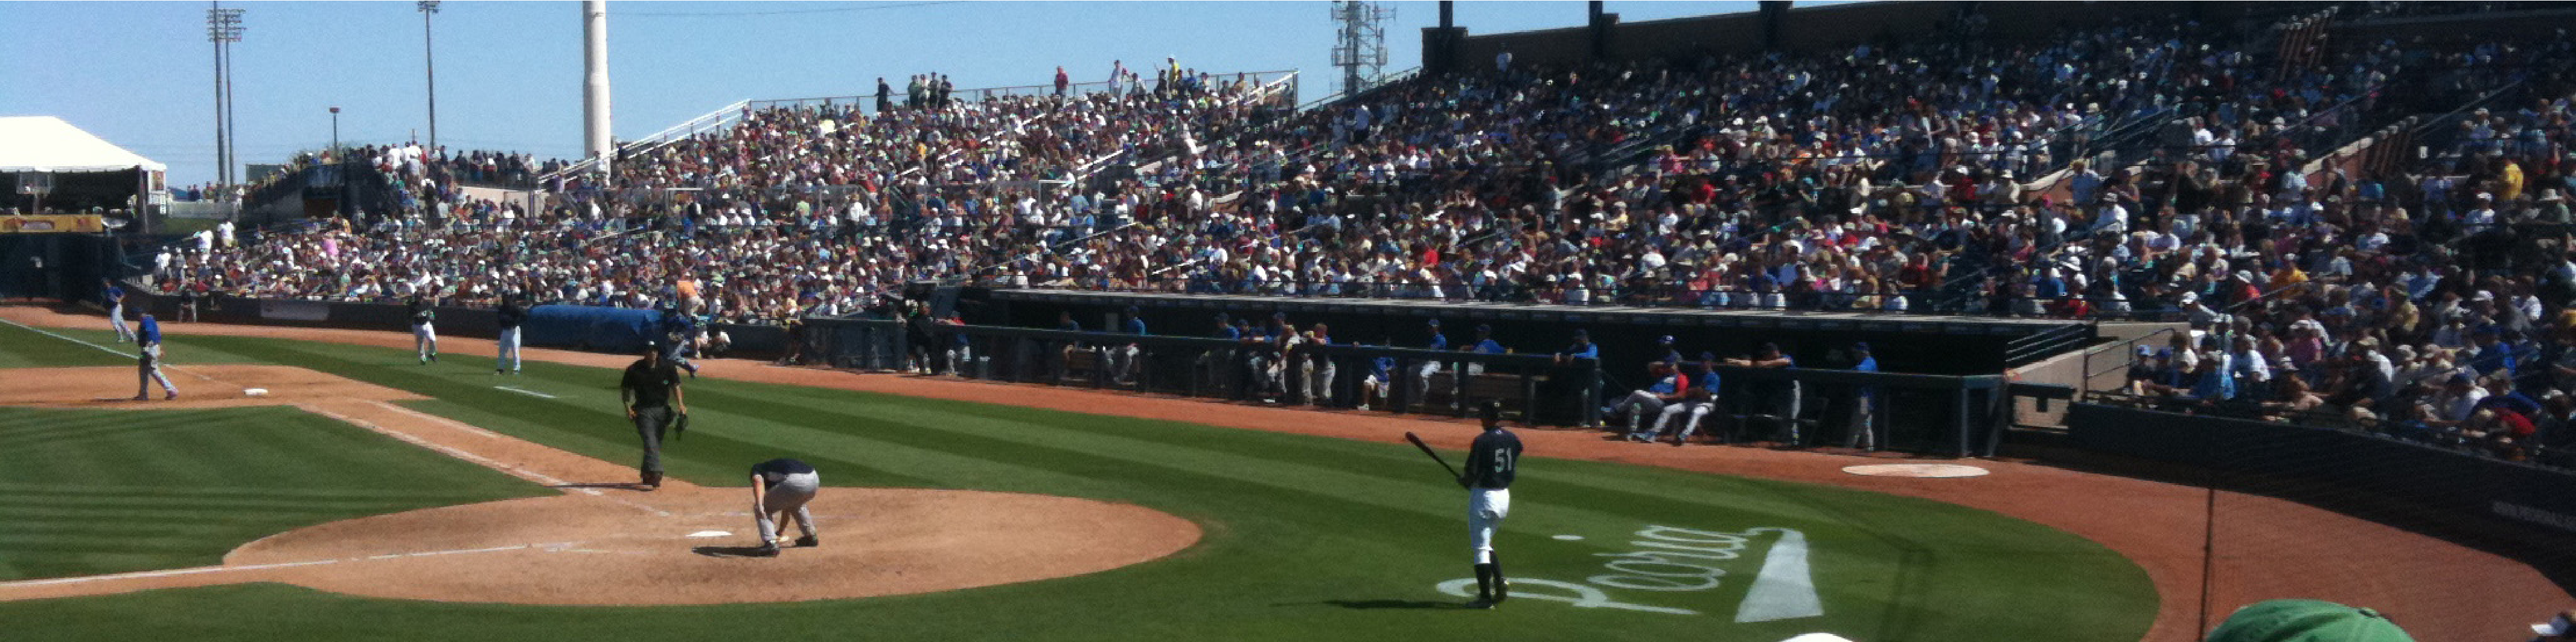
\includegraphics[width=\textwidth]{sampleteaser}
  %%\caption{Seattle Mariners at Spring Training, 2010.}
  %%\Description{Enjoying the baseball game from the third-base
  %%seats. Ichiro Suzuki preparing to bat.}
  %%\label{fig:teaser}
%%\end{teaserfigure}


%%
%% This command processes the author and affiliation and title
%% information and builds the first part of the formatted document.
\maketitle

\section{Introduction}
Dead code, when unaddressed, can be a significant problem for software development.
If not eliminated by the compiler, dead code can make a program 
larger, especially if there is a substantial amount of dead code within a codebase. In addition, dead code 
can make software arbitrarily slower, with additional computational resources devoted 
to declaring unused variables and empty functions. For these reasons, it is imperative that compilers, at 
a minimum, eliminate chunks of code that are unused and uneeded by the program.

Dead code, as defined in this paper, consists of 
two related but distinct situations. Firstly, code can be considered dead if 
it is never executed at runtime. For example, code inside the 'else' portion 
of an if-else block where the condition is always true would be dead. Secondly, a portion of 
code can be considered dead if the computation performed on those lines is never used anywhere else.
For example, a variable that is declared but never written to or read from can be regarded as dead. 

Our project focuses on adding basic dead code elimination strategies into the compiler 
created in the fourth class project. Our goal is to give the compiler support for eliminating
unreachable code in if branches, for loops, and while loops. In addition, the compiler should 
be able to remove unused variables and other miscellaneous dead code optimizations. 

\section{Implementation}
In this section, we will outline how we implemented the aforementioned code removal functionality.

\subsection{Class and Function Additions}
Several additional functions and classes had to be created to implement our optimization pass.
This section will outline the essential modifications, omitting many details and less critical additions.

\subsubsection{AST.cpp and function.cpp Changes}
The Optimize() function is the most important change to the AST class. The Optimize() function 
calls PerformOptimization() on each function. The PerformOptimization() function calls CanOptimize(), which is a function 
that both optimizes a statement and returns its ability to be optimized. This function is described in more detail in the 
subsequent sections.

\subsubsection{Statement.h Changes}
Within the Statement.h file, several additional functions have been declared, with the most important being 
CanOptimize() and HowToOptimize(). The purpose of these functions is self-explanatory. CanOptimize()
returns whether a statement is able to be optimized. We do not try to optimize most types of statements,
so the function returns false by default. HowToOptimize() tells the rest of the program what must be done to optimize 
the statement. HowToOptimize() returns an $Optimization$, which is an enum with values such as $REMOVE\_LOOP$, $REMOVE\_ELSE$, $NO\_OPTIM$,
and others. 

\subsubsection{Block.cpp Changes}
The CanOptimize() function within Block.cpp is where much of the vital optimization work is done.
As mentioned above, CanOptimize() is defined with statement.h, and its children inherit and can override this function.
Though all other subclasses of statement.h simply return a true or false value from the function, the CanOptimize() function 
in Block.cpp will modify the state of the containing block class to reflect the optimization changes. Generally speaking, 
these state changes are the creation and deletion of statements within the statements list.

\subsection{If Statements}
There are two cases where a branch of an if statement will never run. The first case is when the condition 
is always true, regardless of the program's state when the if statement is entered. The second case is when 
the condition is always false.

\subsubsection{Condition Always True}
To check if the condition is always true, we get its compiled R-value. If it is 1, then we know 
the condition must always be true. When this happens, we don't need to have any kind of branching logic in the AST.
All we need to do is generate the code within the else statement and generate the rest of the program like normal. 

\subsubsection{Condition Always Flase}
To check if the condition is always false, we get the compiled R-value of the condition as in the other case. If it is 0, we know 
the condition must always be false. Similarly to the case when the condition is always true, all we must do is generate the code within 
the then statement with no branching logic. 

\subsection{Loops (For And While)}
Just like with the if statements, there are two cases in which a loop may cause dead code. The first case is when the condition 
is always true, and the second case is when the condition is always false.

\subsubsection{Condition Always True}
Just like with if statements, we can check if the condition is always true by looking at its compiled R-value.
If it is 1, then we know that the loop will never terminate, rendering the subsequent code unreachable. To simplify the AST, we can 
eliminate all the following statements after the loop. A return statement is still appended at the end of the loop for consistency's sake,
with the return type matching that of the function. Since the code is unreachable, the value returned is unimportant, and arbitrary
ones were chosen.

\subsubsection{Condition Always False}
If the compiled R-value of the condition is always false, there is no need to include the loop at all within the AST or LLVM IR. 
As such, the entire loop is erased within the AST, with the rest of the code being left unaffected.

\subsection{Useless Variables}
In the end this feature did not end up working as we intended although several different strategies were looked at to do so. 
The first was a flagging method where we would try and flag variables they were defined and only compile those that were flagged. 
We tried to delete variables before compilation that appeared only once in the function. We tried a method where we retroactively 
parsed the compiled file and removed the non-used variables from it. All of these were either wholly
unsuccessful or we didn't have the time to figure them out without major problems.  

\subsection{Other Optimizations}
An additional simple dead code elimination technique is to eliminate adjacent statements.
For example, if the statement $x = 1$ is directly followed by $x = 1$, one of these statements can be removed with 
no effect on the code.

\section{Major Limitations}
There still is a large number of limitations with our optimization pass. This section will outline some of the 
most critical ones.

\subsubsection{Return/break statements within infinite loops}
An infinite loop is not truly infinite if a reachable jumping statement exists within it. 
Our optimization is not able to recognize this, so as long as the condition is always true, it assumes 
the following code is unreachable. 

\subsubsection{Resolving more complicated conditions (specifically in regard to the AST)}
Our optimization pass can only recognize conditions as always being true or false when the condition is either a 
'0' or '1'. Obviously, this is very limiting, as most conditions that are always true/false are more obscure. However, it is worth noting that code has been written that allows IR not to be generated for slightly less 
trivial conditions, such as when a variable is assigned to 0 and then used in the condition. 
Since the optimization pass is only supposed to operate on the AST, this logic has been commented out. See for.cpp, while.cpp, and 
if.cpp for how this is done.


\section{Testing Methodology}
To test our optimization pass, several simple tests were created. The primary metric 
we decided to use to determine the effectiveness of our optimization pass was the size of the generated 
LLVM IR in bytes. For many of our tests, we also recorded execution time. This metric was omitted 
for tests containing infinite loops which last forever.



\section{Results}
Below, you can see space and speed metrics on a small sample of test files. These test files can 
be found in the implementation submission.
As can be seen, our optimization pass had a major impact on the resulting LLVM IR file size, with the 
optimized file being anywhere from 80\% to 35\% of the original file's size. 

Also, there was not a significant impact on speed, but this is likely because the sample files tested were so 
short and straightforward. If a follow-up report were to be produced, we would have created a more 
elaborate testing suite to investigate the performance of our optimization pass on more complex 
pieces of code. The testing suite could include many files with a large number of loops to be 
eliminated and conditional branches that can be pruned.



\begin{table*}
  \caption{File Size Test Results}
  \begin{tabular}{ccl}
    \toprule
    File & Unoptimized IR Size & Optimized IR Size \\
    \midrule
    \texttt{$if\_remove\_then.c$}& 848& 348 \\
    \texttt{$if\_remove\_else.c$}&  847& 348\\
    \texttt{$infinite\_for.c$}& 905& 716 \\
    \texttt{$useless\_for.c$}& 936& 321  \\
    \texttt{$infinite\_while.c$}& 888 & 699 \\
    \texttt{$useless\_while.c$}& 833 & 321  \\
    \bottomrule
  \end{tabular}
\end{table*}

\begin{table*}
  \caption{File Execution Time Test Results}
  \label{tab:commands}
  \begin{tabular}{ccl}
    \toprule
    File & Unoptimized IR Size & Optimized IR Size \\
    \midrule
    \texttt{$if\_remove\_then.c$}& 0.009s & 0.030s \\
    \texttt{$if\_remove\_else.c$}&  0.010s & 0.009s \\
    \texttt{$useless\_for.c$}& 0.009s & 0.009s  \\
    \texttt{$useless\_while.c$}& 0.012s &  0.009s \\
    \bottomrule
  \end{tabular}
\end{table*}

\section{Conclusion}
Though our optimization pass has much room for improvement, it is able to recognize 
and eliminate obvious pieces of dead code, such as unnecessary conditional branches, 
useless loops, and more. Based on the testing results, we can confidently say that the removal of obvious dead code 
can substantially lower the size of the outputted program. In the real world, most 
dead code isn't so simple and easy to recognize, but our project serves as a 
proof-of-concept of the usefulness of dead code removal tools and optimizations. 

\end{document}
\endinput
%%
%% End of file `sample-lualatex.tex'.
